% Options for packages loaded elsewhere
\PassOptionsToPackage{unicode}{hyperref}
\PassOptionsToPackage{hyphens}{url}
\PassOptionsToPackage{dvipsnames,svgnames,x11names}{xcolor}
%
\documentclass[
  number,
  preprint,
  3p,
  onecolumn]{elsarticle}

\usepackage{amsmath,amssymb}
\usepackage{iftex}
\ifPDFTeX
  \usepackage[T1]{fontenc}
  \usepackage[utf8]{inputenc}
  \usepackage{textcomp} % provide euro and other symbols
\else % if luatex or xetex
  \usepackage{unicode-math}
  \defaultfontfeatures{Scale=MatchLowercase}
  \defaultfontfeatures[\rmfamily]{Ligatures=TeX,Scale=1}
\fi
\usepackage{lmodern}
\ifPDFTeX\else  
    % xetex/luatex font selection
\fi
% Use upquote if available, for straight quotes in verbatim environments
\IfFileExists{upquote.sty}{\usepackage{upquote}}{}
\IfFileExists{microtype.sty}{% use microtype if available
  \usepackage[]{microtype}
  \UseMicrotypeSet[protrusion]{basicmath} % disable protrusion for tt fonts
}{}
\makeatletter
\@ifundefined{KOMAClassName}{% if non-KOMA class
  \IfFileExists{parskip.sty}{%
    \usepackage{parskip}
  }{% else
    \setlength{\parindent}{0pt}
    \setlength{\parskip}{6pt plus 2pt minus 1pt}}
}{% if KOMA class
  \KOMAoptions{parskip=half}}
\makeatother
\usepackage{xcolor}
\setlength{\emergencystretch}{3em} % prevent overfull lines
\setcounter{secnumdepth}{5}
% Make \paragraph and \subparagraph free-standing
\makeatletter
\ifx\paragraph\undefined\else
  \let\oldparagraph\paragraph
  \renewcommand{\paragraph}{
    \@ifstar
      \xxxParagraphStar
      \xxxParagraphNoStar
  }
  \newcommand{\xxxParagraphStar}[1]{\oldparagraph*{#1}\mbox{}}
  \newcommand{\xxxParagraphNoStar}[1]{\oldparagraph{#1}\mbox{}}
\fi
\ifx\subparagraph\undefined\else
  \let\oldsubparagraph\subparagraph
  \renewcommand{\subparagraph}{
    \@ifstar
      \xxxSubParagraphStar
      \xxxSubParagraphNoStar
  }
  \newcommand{\xxxSubParagraphStar}[1]{\oldsubparagraph*{#1}\mbox{}}
  \newcommand{\xxxSubParagraphNoStar}[1]{\oldsubparagraph{#1}\mbox{}}
\fi
\makeatother


\providecommand{\tightlist}{%
  \setlength{\itemsep}{0pt}\setlength{\parskip}{0pt}}\usepackage{longtable,booktabs,array}
\usepackage{calc} % for calculating minipage widths
% Correct order of tables after \paragraph or \subparagraph
\usepackage{etoolbox}
\makeatletter
\patchcmd\longtable{\par}{\if@noskipsec\mbox{}\fi\par}{}{}
\makeatother
% Allow footnotes in longtable head/foot
\IfFileExists{footnotehyper.sty}{\usepackage{footnotehyper}}{\usepackage{footnote}}
\makesavenoteenv{longtable}
\usepackage{graphicx}
\makeatletter
\newsavebox\pandoc@box
\newcommand*\pandocbounded[1]{% scales image to fit in text height/width
  \sbox\pandoc@box{#1}%
  \Gscale@div\@tempa{\textheight}{\dimexpr\ht\pandoc@box+\dp\pandoc@box\relax}%
  \Gscale@div\@tempb{\linewidth}{\wd\pandoc@box}%
  \ifdim\@tempb\p@<\@tempa\p@\let\@tempa\@tempb\fi% select the smaller of both
  \ifdim\@tempa\p@<\p@\scalebox{\@tempa}{\usebox\pandoc@box}%
  \else\usebox{\pandoc@box}%
  \fi%
}
% Set default figure placement to htbp
\def\fps@figure{htbp}
\makeatother

\usepackage{booktabs}
\usepackage{longtable}
\usepackage{array}
\usepackage{multirow}
\usepackage{wrapfig}
\usepackage{float}
\usepackage{colortbl}
\usepackage{pdflscape}
\usepackage{tabu}
\usepackage{threeparttable}
\usepackage{threeparttablex}
\usepackage[normalem]{ulem}
\usepackage{makecell}
\usepackage{xcolor}
\makeatletter
\@ifpackageloaded{caption}{}{\usepackage{caption}}
\AtBeginDocument{%
\ifdefined\contentsname
  \renewcommand*\contentsname{Table of contents}
\else
  \newcommand\contentsname{Table of contents}
\fi
\ifdefined\listfigurename
  \renewcommand*\listfigurename{List of Figures}
\else
  \newcommand\listfigurename{List of Figures}
\fi
\ifdefined\listtablename
  \renewcommand*\listtablename{List of Tables}
\else
  \newcommand\listtablename{List of Tables}
\fi
\ifdefined\figurename
  \renewcommand*\figurename{Figure}
\else
  \newcommand\figurename{Figure}
\fi
\ifdefined\tablename
  \renewcommand*\tablename{Table}
\else
  \newcommand\tablename{Table}
\fi
}
\@ifpackageloaded{float}{}{\usepackage{float}}
\floatstyle{ruled}
\@ifundefined{c@chapter}{\newfloat{codelisting}{h}{lop}}{\newfloat{codelisting}{h}{lop}[chapter]}
\floatname{codelisting}{Listing}
\newcommand*\listoflistings{\listof{codelisting}{List of Listings}}
\makeatother
\makeatletter
\makeatother
\makeatletter
\@ifpackageloaded{caption}{}{\usepackage{caption}}
\@ifpackageloaded{subcaption}{}{\usepackage{subcaption}}
\makeatother
\journal{Journal of Environmental Management}

\usepackage[]{natbib}
\bibliographystyle{elsarticle-num}
\usepackage{bookmark}

\IfFileExists{xurl.sty}{\usepackage{xurl}}{} % add URL line breaks if available
\urlstyle{same} % disable monospaced font for URLs
\hypersetup{
  pdftitle={Mapping landscape suitability for forest thinning to reduce evapotranspiration and enhance groundwater recharge in Arizona},
  pdfauthor={Ryan E Lima; Neha Gupta; Travis Zalesky; Temuulen Tsagaan Sankey; Abraham E Springer; Katherine Jacobs},
  pdfkeywords={Suitability mapping, Forest thinning, Water
Resources, Groundwater recharge, Potential Recharge
Zones, GIS-MCDA, WLC},
  colorlinks=true,
  linkcolor={blue},
  filecolor={Maroon},
  citecolor={Blue},
  urlcolor={Blue},
  pdfcreator={LaTeX via pandoc}}


\setlength{\parindent}{6pt}
\begin{document}

\begin{frontmatter}
\title{Mapping landscape suitability for forest thinning to reduce
evapotranspiration and enhance groundwater recharge in Arizona}
\author[1]{Ryan E Lima%
\corref{cor1}%
}
 \ead{ryan.lima@nau.edu} 
\author[2]{Neha Gupta%
%
}

\author[2]{Travis Zalesky%
%
}

\author[1]{Temuulen Tsagaan Sankey%
%
}

\author[1]{Abraham E Springer%
%
}

\author[2]{Katherine Jacobs%
%
}


\affiliation[1]{organization={Northern Arizona
University},,postcodesep={}}
\affiliation[2]{organization={University of Arizona},,postcodesep={}}

\cortext[cor1]{Corresponding author}






        
\begin{abstract}
Literature on the relationship between forest thinning and water yield
was used to develop suitability criteria to map where forest treatment
is most likely to enhance groundwater recharge across the Ponderosa Pine
(\emph{Pinus ponderosa}) forests of Arizona. Recharge in Ponderosa Pine
forests is ephemeral and focused in periods of snowmelt and locations of
enhanced permeability when soil moisture exceeds threshold levels. Our
approach combines thematic maps of criteria such as snow dominance,
slope, aspect, landscape morphology, forest basal area, canopy cover,
lineament density, lithology, and hydrologic soil type into a
GIS-Multi-Criteria Decision Analysis (GIS-MCDA) model. Individual
criteria were grouped into indices using Weighted Linear Combinations
(WLC). A total of 863,648 hectares or 46.8\% of the 1.8 million hectares
of Ponderosa Pine forests were found to be highly suitable for
groundwater recharge enhancement from forest thinning. Similar
approaches and criteria selection can be applied to other areas in the
Southwestern US and other forest types to identify areas for forest
thinning for potential recharge benefits.
\end{abstract}





\begin{keyword}
    Suitability mapping \sep Forest thinning \sep Water
Resources \sep Groundwater recharge \sep Potential Recharge
Zones \sep GIS-MCDA \sep 
    WLC
\end{keyword}
\end{frontmatter}
    

\section{Introduction}\label{introduction}

Warming associated with anthropogenic climate change has led to a
doubling in the frequency of extreme hydroclimate events in the Colorado
River Basin since 2010, including droughts, heatwaves, and floods
\citep{bennett_concurrent_2021}. Since 2000, the Colorado River Basin
has experienced a historic drought
\citep{meko_treering_2022, williams_rapid_2022}. Over this time period,
streamflow in the Colorado River has declined by 19\% (3.6E9 \(m^3\))
relative to the 1906-1999 average (18.7E10 \(m^3\));
\citep{hogan_recent_2024, udall_twentyfirst_2017}. Rapid population
growth in the Southwest and Arizona, in particular, is increasing the
demands on already strained water supplies in the State. Reductions in
streamflow have increased reliance on groundwater pumping, resulting in
groundwater declines across Arizona \citep{tadych_historical_2024}.
Analyses of regional gravity data have suggested that groundwater loss
rate in the Colorado River Basin may far exceed the depletion rate of
Lake Powell and Lake Mead and that groundwater may account for a more
significant portion of water use than previously thought
\citep{castle2014}.

Warming temperatures have also tripled the frequency and quadrupled the
size of wildfires since 2000 \citep{iglesias2022}. The risk of
catastrophic wildfires is increasing in Western forests--an emerging
driver of runoff change that will increase the impact on the water
supply \citep{williams_rapid_2022}. Forest structure in Northern Arizona
has changed significantly post-Euro-American settlement. Many forests
are overstocked relative to pre-settlement conditions due to grazing,
logging, and wildfire exclusion
\citep{covington_southwestern_1994, friederici2013}. These changes have
increased the risk of catastrophic wildfires \citep{allen2002}. Rising
temperatures and droughts have contributed to extensive tree mortality
from disease and insect infestation, making forested areas more
vulnerable to wildfires \citep{berner_tree_2017}.

Forest treatments such as thinning and prescribed burning can
significantly impact the hydrologic cycle of forests
\citep{del_campo_global_2022}. For example, forest thinning in Arizona
has been associated with increased snow cover days
\citep{sankey_multi-scale_2015, belmonte2021, donager_integrating_2021},
greater soil moisture \citep{belmonte_soil_2022, sankey_thinning_2022},
and greater forest canopy moisture \citep{sankey_regionalscale_2021}.

Numerous studies have linked forest treatments to increased water yields
in semi-arid forests and have emphasized the role of forest restoration
in improving hydrologic services and increasing water availability
\citep{bosch1982, baker_effects_1986, gottfried_moderate_1991, smerdon_overview_2009, zou_streamflow_2010, wyatt2013, moreno_modeling_2015, simonit_impact_2015, wyatt2015, odonnell_forest_2018, schenk_impacts_2020, hibbert1979}.
While the connection between forest treatment and water yield is well
documented, the response of forests to treatments is complex and
non-linear and differs across forest types, with treatment level, and
along aspect and elevational gradients
\citep{del_campo_global_2022, biederman2022, zou_streamflow_2010, hibbert1979, moore2005};.

Regardless of the potential for increased water yield, the enhancement
of groundwater recharge rarely, if ever, ranks among the primary
motivations for forest treatment, even among projects with the stated
goal of improving watershed health
\citep{stanturf2014, filoso2017, allen2002, friederici2013, odonnell2016}.
Studies that surveyed public willingness to pay for forest restoration
to enhance groundwater recharge were the lowest among the environmental
services discussed in the survey, behind critical habitat protections,
surface water quality improvements, and preservation of cultural
values\citep{mueller2019, soder2022}. This suggests that groundwater
recharge is either undervalued by the public as an ecosystem service or
a low priority relative to other environmental goods.

Forest health and water security are intimately linked. About 66\% of
the water supply in 11 western states comes from Forested Lands
\citep{brown_source_2005}. Despite this, the management of lands and
waters is still largely compartmentalized. The Western Water Network
(WWN) identified the need to promote better and faster collaboration
between researchers, managers, educators, industry, and stakeholders
across the West \citep{hansen2024}. This study examines forest
restoration through the lens of groundwater recharge enhancement and
aims to identify potential recharge zones. Specifically, we demonstrate
a suitability mapping approach to identify areas where forest thinning
may enhance recharge. Suitability maps like these may complement (or
supplement) existing frameworks for jointly prioritizing landscape-scale
forest management and managing lands and water.

Suitability mapping, particularly GIS-based Multi-criteria decision
analysis (GIS-MCDA) and Analytic Hierarchy Process (AHP), have been
widely used to map potential recharge zones and areas suitable for
Managed Aquifer Recharge (MAR) in areas underlain by karst lithologies
\citep{fathi2021, rajashekar2023, rahman2012, dar2020, shaban2006}.
However this study is the first to examine where forest restoration may
be sited to enhance un-managed recharge at a landscape scale. This study
finds that much of the area where thinning is planned for the purpose of
restoring other ecosystem services may also improve groundwater
management in a state facing serious groundwater declines.

\subsection{Study Area}\label{study-area}

Our study area includes all of the HUC8 watersheds of Arizona, extending
into 5 other states but excluding Mexico. However within that study area
we focus on the Ponderosa Pine woodland type. Ponderosa Pine woodlands
cover 1.8 million hectares (1,835,530.65) of this study area or around
30\% (28.38\%) of the forested area within its bounds. Most of the
ponderosa pine forest is found along the Mogollon Rim, around the San
Francisco Peaks, and on the Kaibab Plateau--all within the Colorado
Plateau physiographic region at elevations between 2000 \(m\) and 2400
\(m\). Smaller isolated patches of Ponderosa Pine forest can be found on
mountain ranges and plateaus throughout Arizona at similar elevations
(see Figure~\ref{fig-studyarea} ).

The Mogollon Rim is a topographic feature forming the southern edge of
the Colorado Plateau. It contains the majority of the state's ponderosa
pine forests and has been identified as an essential groundwater
recharge area for regional aquifers \citep{parker2005}. Of the estimated
2.1 billion \(m^3\) (174,000 acre-feet) of precipitation that falls on
the Mogollon Rim, about 8\% is estimated to recharge the regional
groundwater aquifers\citep{parker2005} Similarly, The Kaibab Plateau, an
uplifted region north of the Grand Canyon with large stands of ponderosa
pine, is a critically important recharge area for springs in the Grand
Canyon which provide the sole source of drinking water for over 6
million annual visitors and the residents of the National
Park\citep{tobin2018}. The Kaibab plateau lacks perennial surface
streams and is drained rapidly by sinkholes, faults, and fractures or
more slowly through diffuse infiltration with little streamflow leaving
the plateau \citep{jones2018, huntoon1974}.

Most of the Ponderosa Pine forest within the State is within the Kaibab,
Coconino, Apache-Sitgreaves, and Tonto National Forests. Precipitation
in Arizona is bi-modal, with wet winters and a late-summer monsoon
season. As much as 60\% of precipitation at elevations above 1800 m
comes in the form of snow, and snow is responsible for 80 - 95\% of
streamflow and much of the recharge
\citep{baker2013, eastoe2023, earman2006}. Therefore, this research
focuses on high-elevation (\textgreater1800 m) ponderosa pine forests,
which receive a high proportion of annual precipitation as snow. Of the
1.8 million Ha of Ponderosa pine forests in our study area, about 43\%
or 786,706 hectares are underlain by lithologies that may support karst
or pseudo karst features, including carbonates (24\%), evaporates (6\%),
and fractured volcanics (13\%). These areas merit extra attention due to
enhanced infiltration potential through fractures, faults, lava tubes,
or sinkholes.

\begin{figure}

\centering{

\pandocbounded{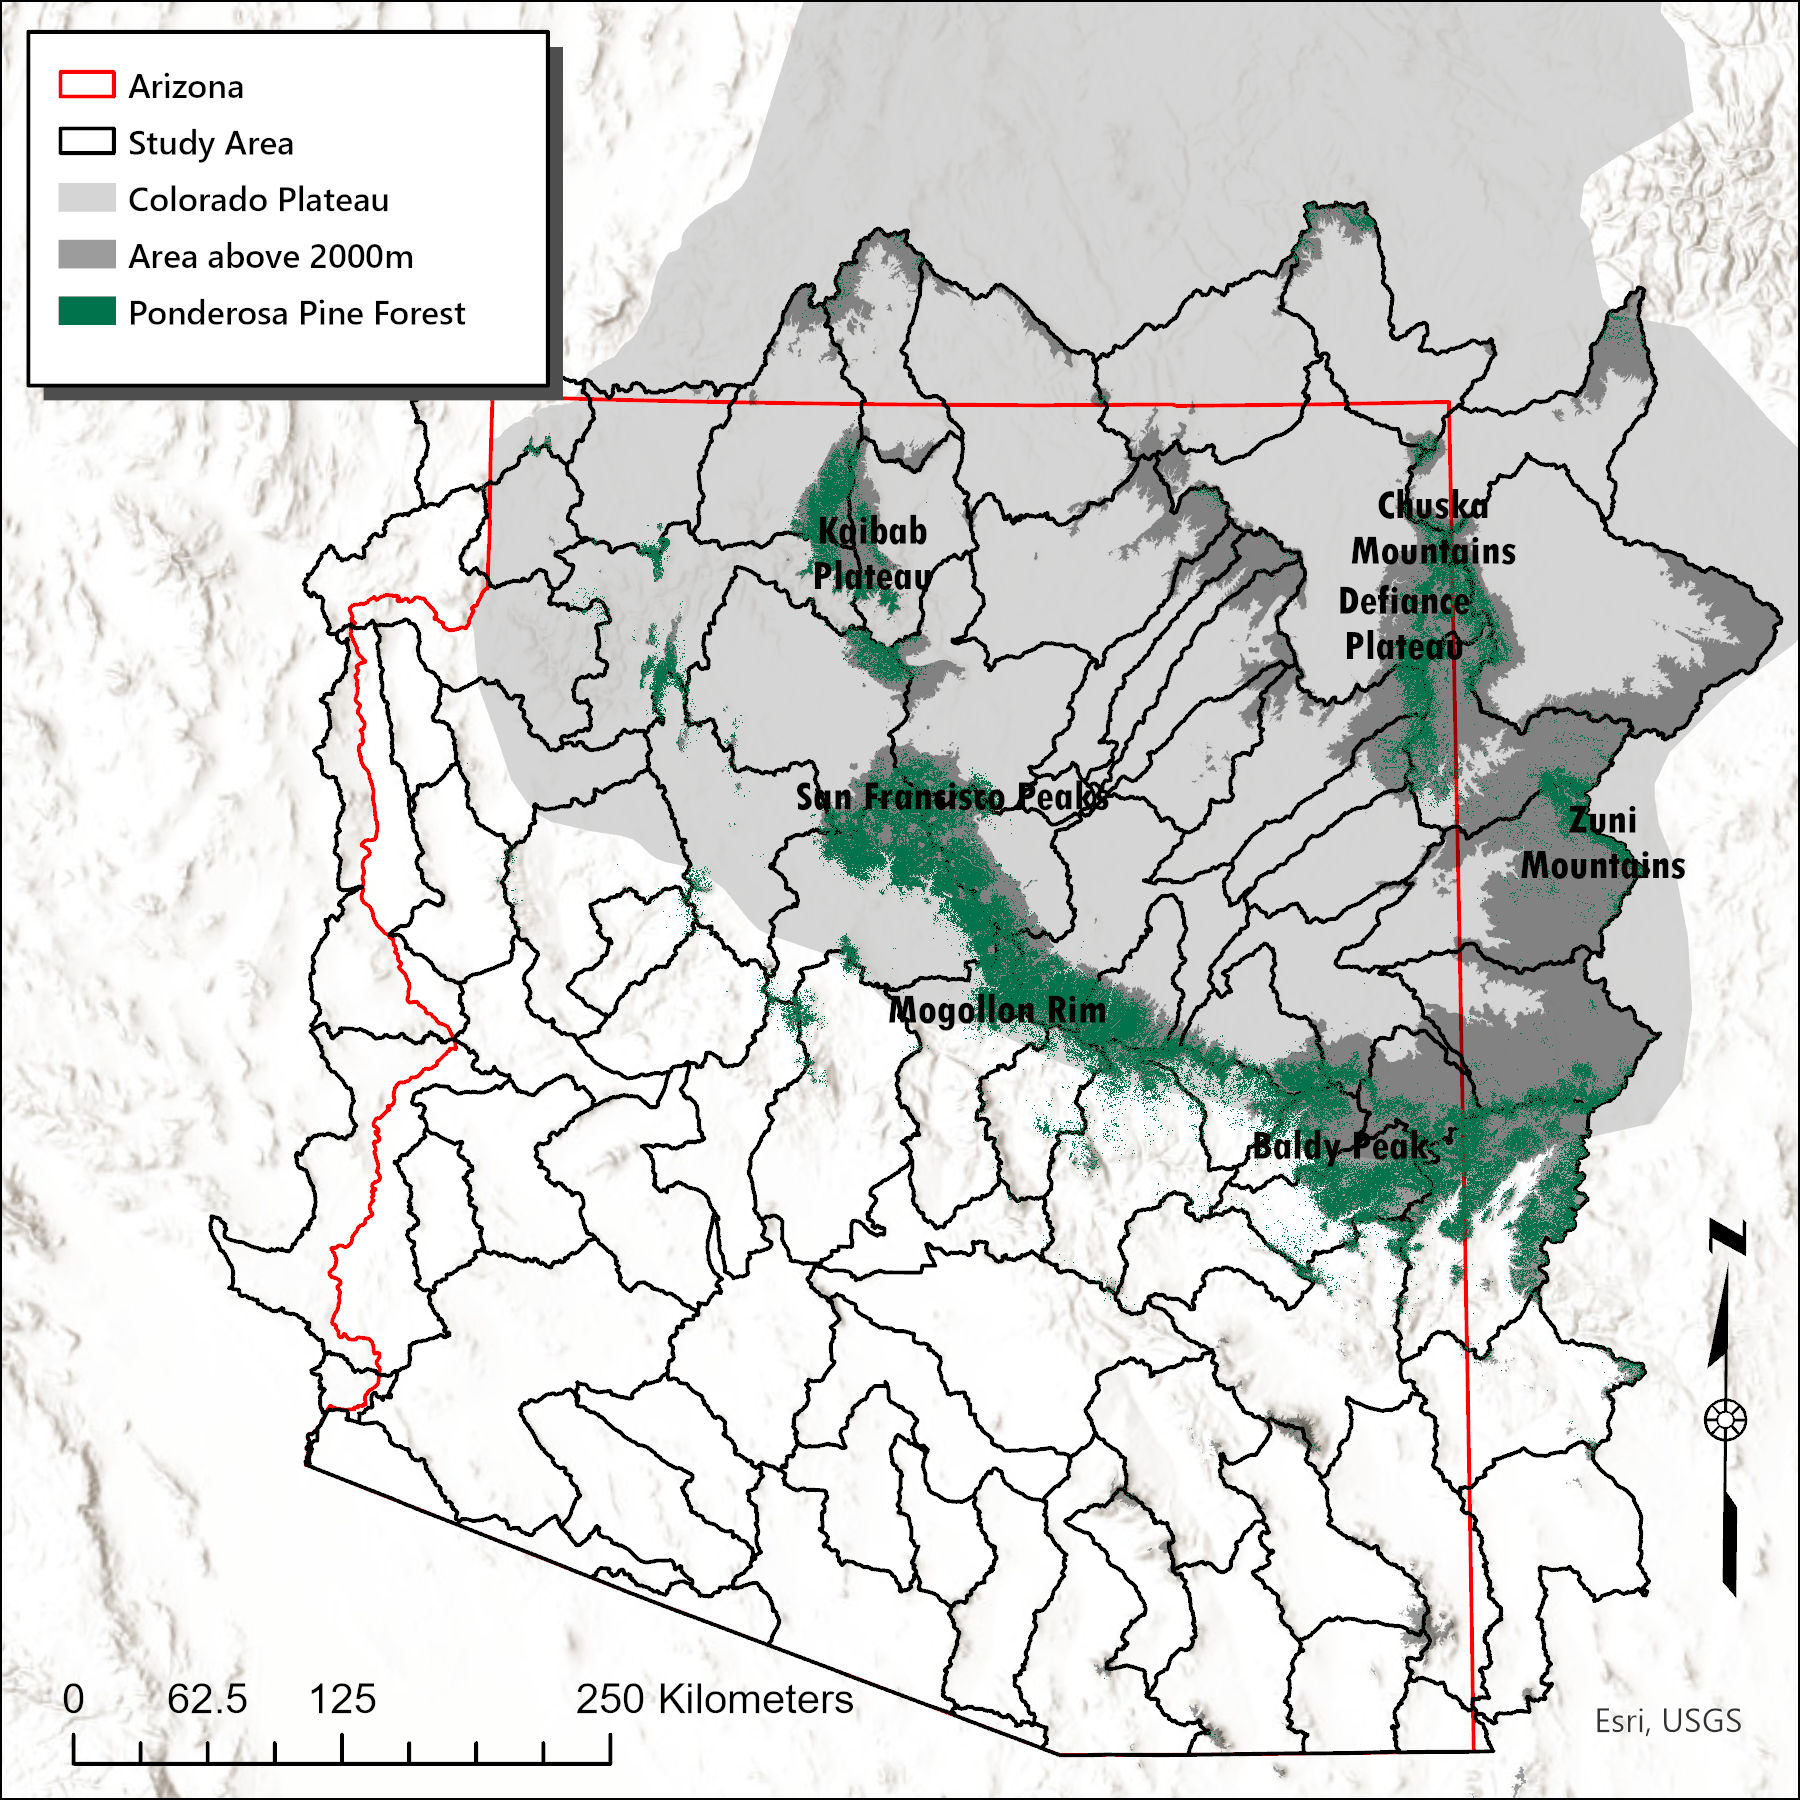
\includegraphics[keepaspectratio]{images/Study_area_map.jpg}}

}

\caption{\label{fig-studyarea}This is a map showing the extent of our
study area and the distribution of Ponderosa pine-dominant forests. The
Colorado Plateau physiographic province is shown in light grey, while
areas within our study area at elevations above 2000m are shown in dark
grey. The HUC8 watersheds are shown in black, and the boundary of
Arizona is shown in Red.}

\end{figure}%

\subsection{Literature Review and
Criteria}\label{literature-review-and-criteria}

This research aims to identify areas where mechanical thinning is most
likely to enhance groundwater recharge. We based our suitability
criteria on literature primarily from regional studies, as they are
likely the best predictors of hydrologic response to thinning in
Arizona's forests \citep{wyatt_estimating_2013}. Landscape-scale forest
restoration efforts have been planned or implemented across much of
Arizona. For example, the Four Forest Restoration Initiative (4FRI)
includes plans for restoration across over 1 million hectares of
Arizona's forests \citep{schultz_collaborative_2012}. A synthesis of
4FRI treatments found that thinned and burned forests have significantly
greater total ecosystem moisture and are thus more resilient to drought
and wildfire \citep{sankey_thinning_2022, sankey_regionalscale_2021}.
Thinned forests also have more snow and soil moisture
\citep{odonnell_vegetation_2021, belmonte_soil_2022}.

The snow and its persistence appear particularly important for recharge
in Arizona's semi-arid and high-elevation conifer forests. Analysis of
groundwater issuing from springs along the Mogollon rim found a strong
relationship between snow persistence and the duration of spring
discharge \citep{donovan2022}. Isotopic groundwater analyses have
revealed that Northern Arizona's recharge is dominated by winter
precipitation from altitudes above 1500
m\citep{eastoe2007, eastoe2023, earman2006, blasch2006}. Studies of
plant water use have found that larger ponderosa pine trees primarily
utilize deeper soil moisture from winter precipitation, while understory
vegetation and smaller trees utilize shallow soil water from monsoonal
storms, informing our approach to focusing on ponderosa pine trees for
this analysis \citep{kerhoulas2013, kerhoulas2023}.

Thinning in Ponderosa Pine forests is expected to increase available
water in two primary ways. 1) reducing transpiration of deep soil water
by overstory vegetation and 2) reducing canopy interception of snow and
subsequent sublimation, increasing below-canopy snow depth and snow
persistence. Thinning in semi-arid forested watersheds can significantly
alter snowmelt timing \citep{dwivedi2024}. Reduced forest cover can
delay snowmelt at colder sites, higher elevations, and northern aspects
or advance snowmelt through increasing sub-canopy solar radiation and
wind, particularly at lower elevations, southern aspects, and warmer
sites \citep{biederman_recent_2015, dwivedi2024}.

Total annual precipitation also appears to influence whether thinning
reduces or enhances water yield at particular sites. In the Colorado
River Basin, there appears to be a precipitation threshold at work.
Below \textasciitilde500 \(mm\) of annual precipitation, precipitation,
and runoff may become decoupled \citep{biederman2022}, likely because
below \textasciitilde500 \(mm\), most precipitation is evaporated
regardless of forest condition. Semi-arid forests with high inter-annual
precipitation variability may show effects in wet years when
precipitation is greater than \textasciitilde500 \(mm\) or in
snow-dominant watersheds
\citep{adams_ecohydrological_2012, carroll_evaluating_2016}.

Canopy cover between 25\% and 40\% appears optimal for net snow
accumulation at continental mid-latitude sites \citep{veatch2009}.
UAV-based studies within the study area have shown that 24 - 35\% canopy
cover was optimal for snow persistence.
\citep{donager2021, sankey_multi-scale_2015, belmonte2021}. However,
water yield enhancement from thinning likely requires at least a 20\%
reduction in canopy cover\citep{adams_ecohydrological_2012}. Hydrologic
models in northern Arizona watersheds suggest that reductions in basal
area of at least 30\% can increase groundwater recharge by up to 15\%
\citep{wyatt2015}.

Research on the effect of thinning to below-ground hydrological
processes in semi-arid Mediterranean forests found that sites with high
antecedent soil moisture had the highest response, with drainage to
deeper soil layers increasing by 50 mm/year relative to control
sites\citep{del_campo_effectiveness_2019}. The soil type (texture,
composition, field capacity, and permeability) and topography affect the
soil moisture. Slope, Aspect, landscape convexity or concavity, and
geomorphons (or landform types) such as pits, flats, hills, valleys,
ridges, and hollows strongly affect the accumulation and residence time
of overland flow and shallow soil
water\citep{parker1982, jasiewicz2013}. In dry soils, capillary forces
generally dominate over gravitational forces, and areas with higher flow
accumulation and residence time are more likely to reach field capacity,
leading to more percolation\citep{woessner2020}.

Another important aspect affecting recharge enhancement potential is the
underlying lithology, which controls the subsurface flow of groundwater.
The state currently lacks detailed hydrogeologic mapping. However,
representative ranges of primary (matrix) permeability and porosity
values for rock types are available based on 1:1,000,000 and 1:500,000
geologic mapping data\citep{huscroft2018, freeze1979, woessner2020}.
Secondary permeability and porosity, which involve flow in faults and
fractures, can be estimated to some degree by measuring the density of
linear surface features, or `lineaments,' which often correspond to
underlying geologic structures \citep{oleary1976, sander2007}.
Lineaments have been used to identify potential groundwater supplies,
and studies have found higher well yields along lineaments
\citep{sander2007}. In some crystalline bedrock, groundwater flow occurs
exclusively in faults and fractures \citep{meijerink2007, nyborg2007}.
Orientations of lineaments can help determine the anisotropy of the
fracture environment\citep{meijerink2007}. Caves and sinkholes (or
dolines) often form along and at the intersection of faults and
fractures in karst terrains \citep{ford2007}. Karst and pseudo-karst
terrains can have enhanced infiltration potential far beyond the
hydraulic conductivity of the rock matrix \citep{kresic2013}. For
example, the Edwards Aquifer in Texas was found to have permeability
values that vary by up to nine orders of magnitude \citep{halihan1998}.
The presence or absence of karst or pseudo karst in concert with
lineament density is a critical criterion made explicit in our
suitability analysis.

In summary, suitability for sites where thinning enhances recharge would
most likely occur in areas with significant snowfall, maximum annual
precipitation \textgreater= 500 \(mm\), higher antecedent soil moisture,
NE aspects, in valleys or flat areas where a 20\% reduction in canopy
cover and a 30\% reduction in basal area would result in a thinned
canopy cover of between 25 and 35\%. Suitability would be lowest in
sites with minimal snowfall, SW aspects, lower elevations, ridge tops,
or steep slopes, where thinning might reduce canopy cover to below 24\%.
Soil Hydraulic Conductivity, flow accumulation, and topographic metrics
can reveal the areas likely to have higher antecedent soil moisture.
Lithology, primary permeability and porosity, and lineament density can
provide insight into where rapid subsurface infiltration is possible.

\section{Methods}\label{methods}

\subsection{Suitability Criteria}\label{suitability-criteria}

We used ArcGIS Pro 3.4.0 to create a weighted suitability model
consisting of the 12 thematic data layers shown in
Table~\ref{tbl-thematic} . These were re-scaled, weighted, and combined
into four final thematic layers: (1) Snow Dominance, (2) Vegetation
Density Index, (3) Soil Moisture and Infiltration Index, and (4)
Subsurface Infiltration Index (see Table~\ref{tbl-thematic} ).

\begin{table}

\caption{\label{tbl-thematic}}

\centering{

\pandocbounded{
\includegraphics[keepaspectratio]{index_files/figure-pdf/tbl-thematic-1.png}}


\includegraphics[width=6.19in,height=\textheight,keepaspectratio]{table_screenshot.png}

}

\end{table}%

\textsubscript{Source:
\href{https://Ryan3Lima.github.io/ATUR-Thinning-to-enhance-recharge/index.qmd.html}{Article
Notebook}}

\paragraph{Snowfall Fraction (SF)}\label{snowfall-fraction-sf}

Snowfall Fraction (SF) is the percent of annual precipitation that comes
in the form of snow based on measures of Snow Water Equivalent SWE,
PRISM, and CONUS 404 data produced by the University of Arizona. Snow
has an out-sized role in recharge at elevations over 1800 m in Arizona
\citep{eastoe2007, eastoe2023, baker2013, earman2006} and snow dominance
appears to be an important factor in whether thinning enhances recharge
\citep{adams_ecohydrological_2012, carroll_evaluating_2016, saksa2017}.
Therefore our suitability mapping prioritizes areas with more snowfall
relative to rainfall or higher SF.

\paragraph{Canopy Cover (sCC)}\label{canopy-cover-scc}

Canopy Cover was obtained from the 2021 National Land Cover Database,
which estimates Total Canopy Cover at a 30m resolution. Canopy cover
values ranged from 0\% - 86\%. NLCD Total canopy cover was reclassified
to a 1-10 scale based on suitability for thinning to enhance recharge.
We set a value for 1 for all forests with canopy cover \textless=
12.5\%. This is the minimum required for a 20\% reduction in canopy
cover with a resulting canopy cover \textgreater= the pre-settlement
historic minimum canopy cover of 10\%. Suitability then scales linearly
to 10 for percent cover \textgreater= 28.75\%. Based on the studies
found 23\% to 35\% as the ideal canopy cover range for retaining snow
and a required 20\% reduction in canopy cover. All cells with canopy
cover above 28.75\% are given a 10 for suitability resulting in the
scaled canopy cover (sCC) layer.

\paragraph{Basal Area (sBA)}\label{basal-area-sba}

We extracted basal area estimates from the TreeMap 2016
\citep{riley2022} CONUS dataset with a resolution of 30 meters.
Estimates of pre-settlement ponderosa pine forest basal area were
between 9.2 and 18 \(m^2 ha^-1\) Since basal area reductions of at least
30\% are required to increase water yield. To remove 30\% of the basal
area and have thinned forests remain within the historical range of
pre-settlement forest density all cells with basal areas of 13.14
\(m^2 ha^-1\) or less were given a value of 1, suitability then
increased linearly til it reached 10 at basal areas \textgreater= 25.71
\(m^2 ha^-1\) resulting in the scaled basal area thematic layer (sBA)

\phantomsection\label{cell-fig-veg}
\begin{figure}[H]

\centering{

\pandocbounded{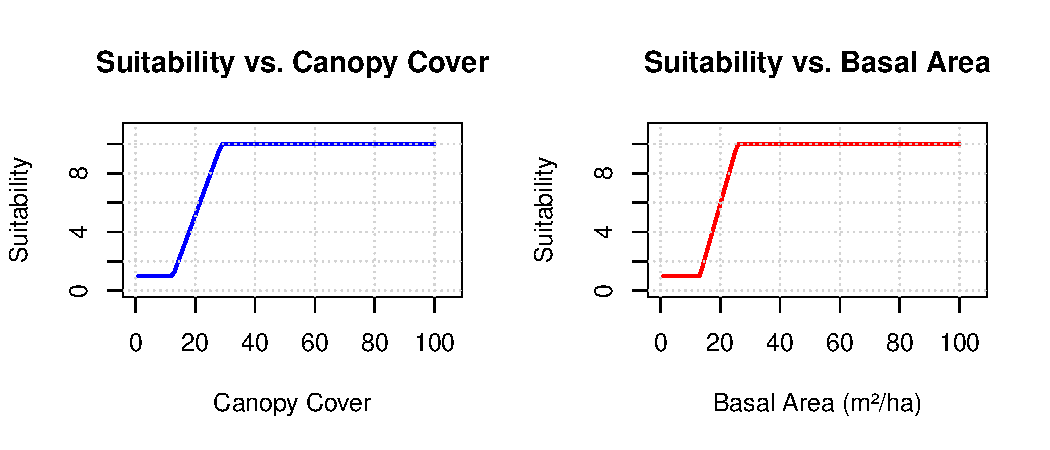
\includegraphics[keepaspectratio]{index_files/figure-pdf/fig-veg-1.pdf}}

}

\caption{\label{fig-veg}Rescaling Canopy Cover and Basal Area for
suitability}

\end{figure}%

\textsubscript{Source:
\href{https://Ryan3Lima.github.io/ATUR-Thinning-to-enhance-recharge/index.qmd.html}{Article
Notebook}}

\subsubsection{Vegetation Density Index
(VDI)}\label{vegetation-density-index-vdi}

Scaled basal area (sBA) and scaled canopy cover (sCC) were combined with
linear weights of 0.6667 and 0.3333, respectively, to create the
vegetation density index (VDI) shown in @eq-vdi. This reflects the fact
that reductions in basal area are more likely correlated with reductions
in ET, while canopy cover primarily affects precipitation partitioning
and sub-canopy solar radiation.

\begin{equation}\phantomsection\label{eq-vdi}{
VDI  = ( sBA* 0.6667)) + (sCC * 0.3333)
}\end{equation}

\paragraph{Soil Hydraulic Conductivity
(SoilKsat)}\label{soil-hydraulic-conductivity-soilksat}

Soil Hydraulic Conductivity (SoilKsat) is used to estimate the max
infiltration rate of the top 2 meters of the soil profile. SoilKsat
comes from the gridded National Soil Geographic Database produced by the
USDA-NRCS. The gNATSGO Soil Hydraulic Conductivity layer provides
estimates of the rate at which water moves through the pores of
saturated soil based on point field measurements of soil texture,
structure, and porosity. Data was aggregated for the AZHUC8 study area
using the Weighted Average method for soil layers from 0 - 200 cm, using
the Soil Data Development Toolbox in ArcMap 10.8.3. Values are reported
in micrometers per second and broken into the standard 6 classes from
very low (0.00 - 0.01) to Very High (100 - 705)

\paragraph{Topographic Relative Moisture Index
(TRMI)}\label{topographic-relative-moisture-index-trmi}

Topographic Relative Moisture Index (TRMI) incorporates several
topographic parameters that influence moisture dynamics, including slope
gradient, aspect, relative elevation (or topographic position), and
landscape convexity or concavity \citep{parker1982}.TRMI was calculated
by ranking Slope (degrees) (1-10), Slope Configuration (Topographic
Position Index) (1-10), Geomorphon (ArcGIS Pro 3.4.0 Spatial Analyst
Toolbox--Geomorphon Landform Tool) (1-20), and aspect (degrees azimuth)
(1-20). Values were summed to calculate a TRMI score between 4 and 60,
classified into 10-classes with equal intervals.

\subsubsection{Soil Moisture and Infiltration Index
(SMII)}\label{soil-moisture-and-infiltration-index-smii}

The Soil Moisture and Infiltration Index (SMII) represents where water
accumulates and is retained on the landscape and where it is likely to
infiltrate through the top 2 meters of the soil profile. This index is a
weighted linear combination of the Topographic Relative Moisture Index
and Soil Saturated Hydraulic Conductivity see Figure~\ref{fig-soil}. The
weights were determined by ranking the variables of relative importance
to each other. Using a top-down approach, we prioritized supply over
infiltration, reasoning that infiltration matters less in areas where
there is no accumulated water to infiltrate. Therefore we applied a
weight of 0.6667 to TRMI and 0.3333 to Soil Saturated Hydraulic
Conductivity (SoilKsat). The weighted linear combination is shown in
Equation~\ref{eq-smii} .

\begin{equation}\phantomsection\label{eq-smii}{
SMII = (TRMI * (0.6667)) + (SoilK) * (0.3333))
}\end{equation}

\begin{figure}

\centering{

\pandocbounded{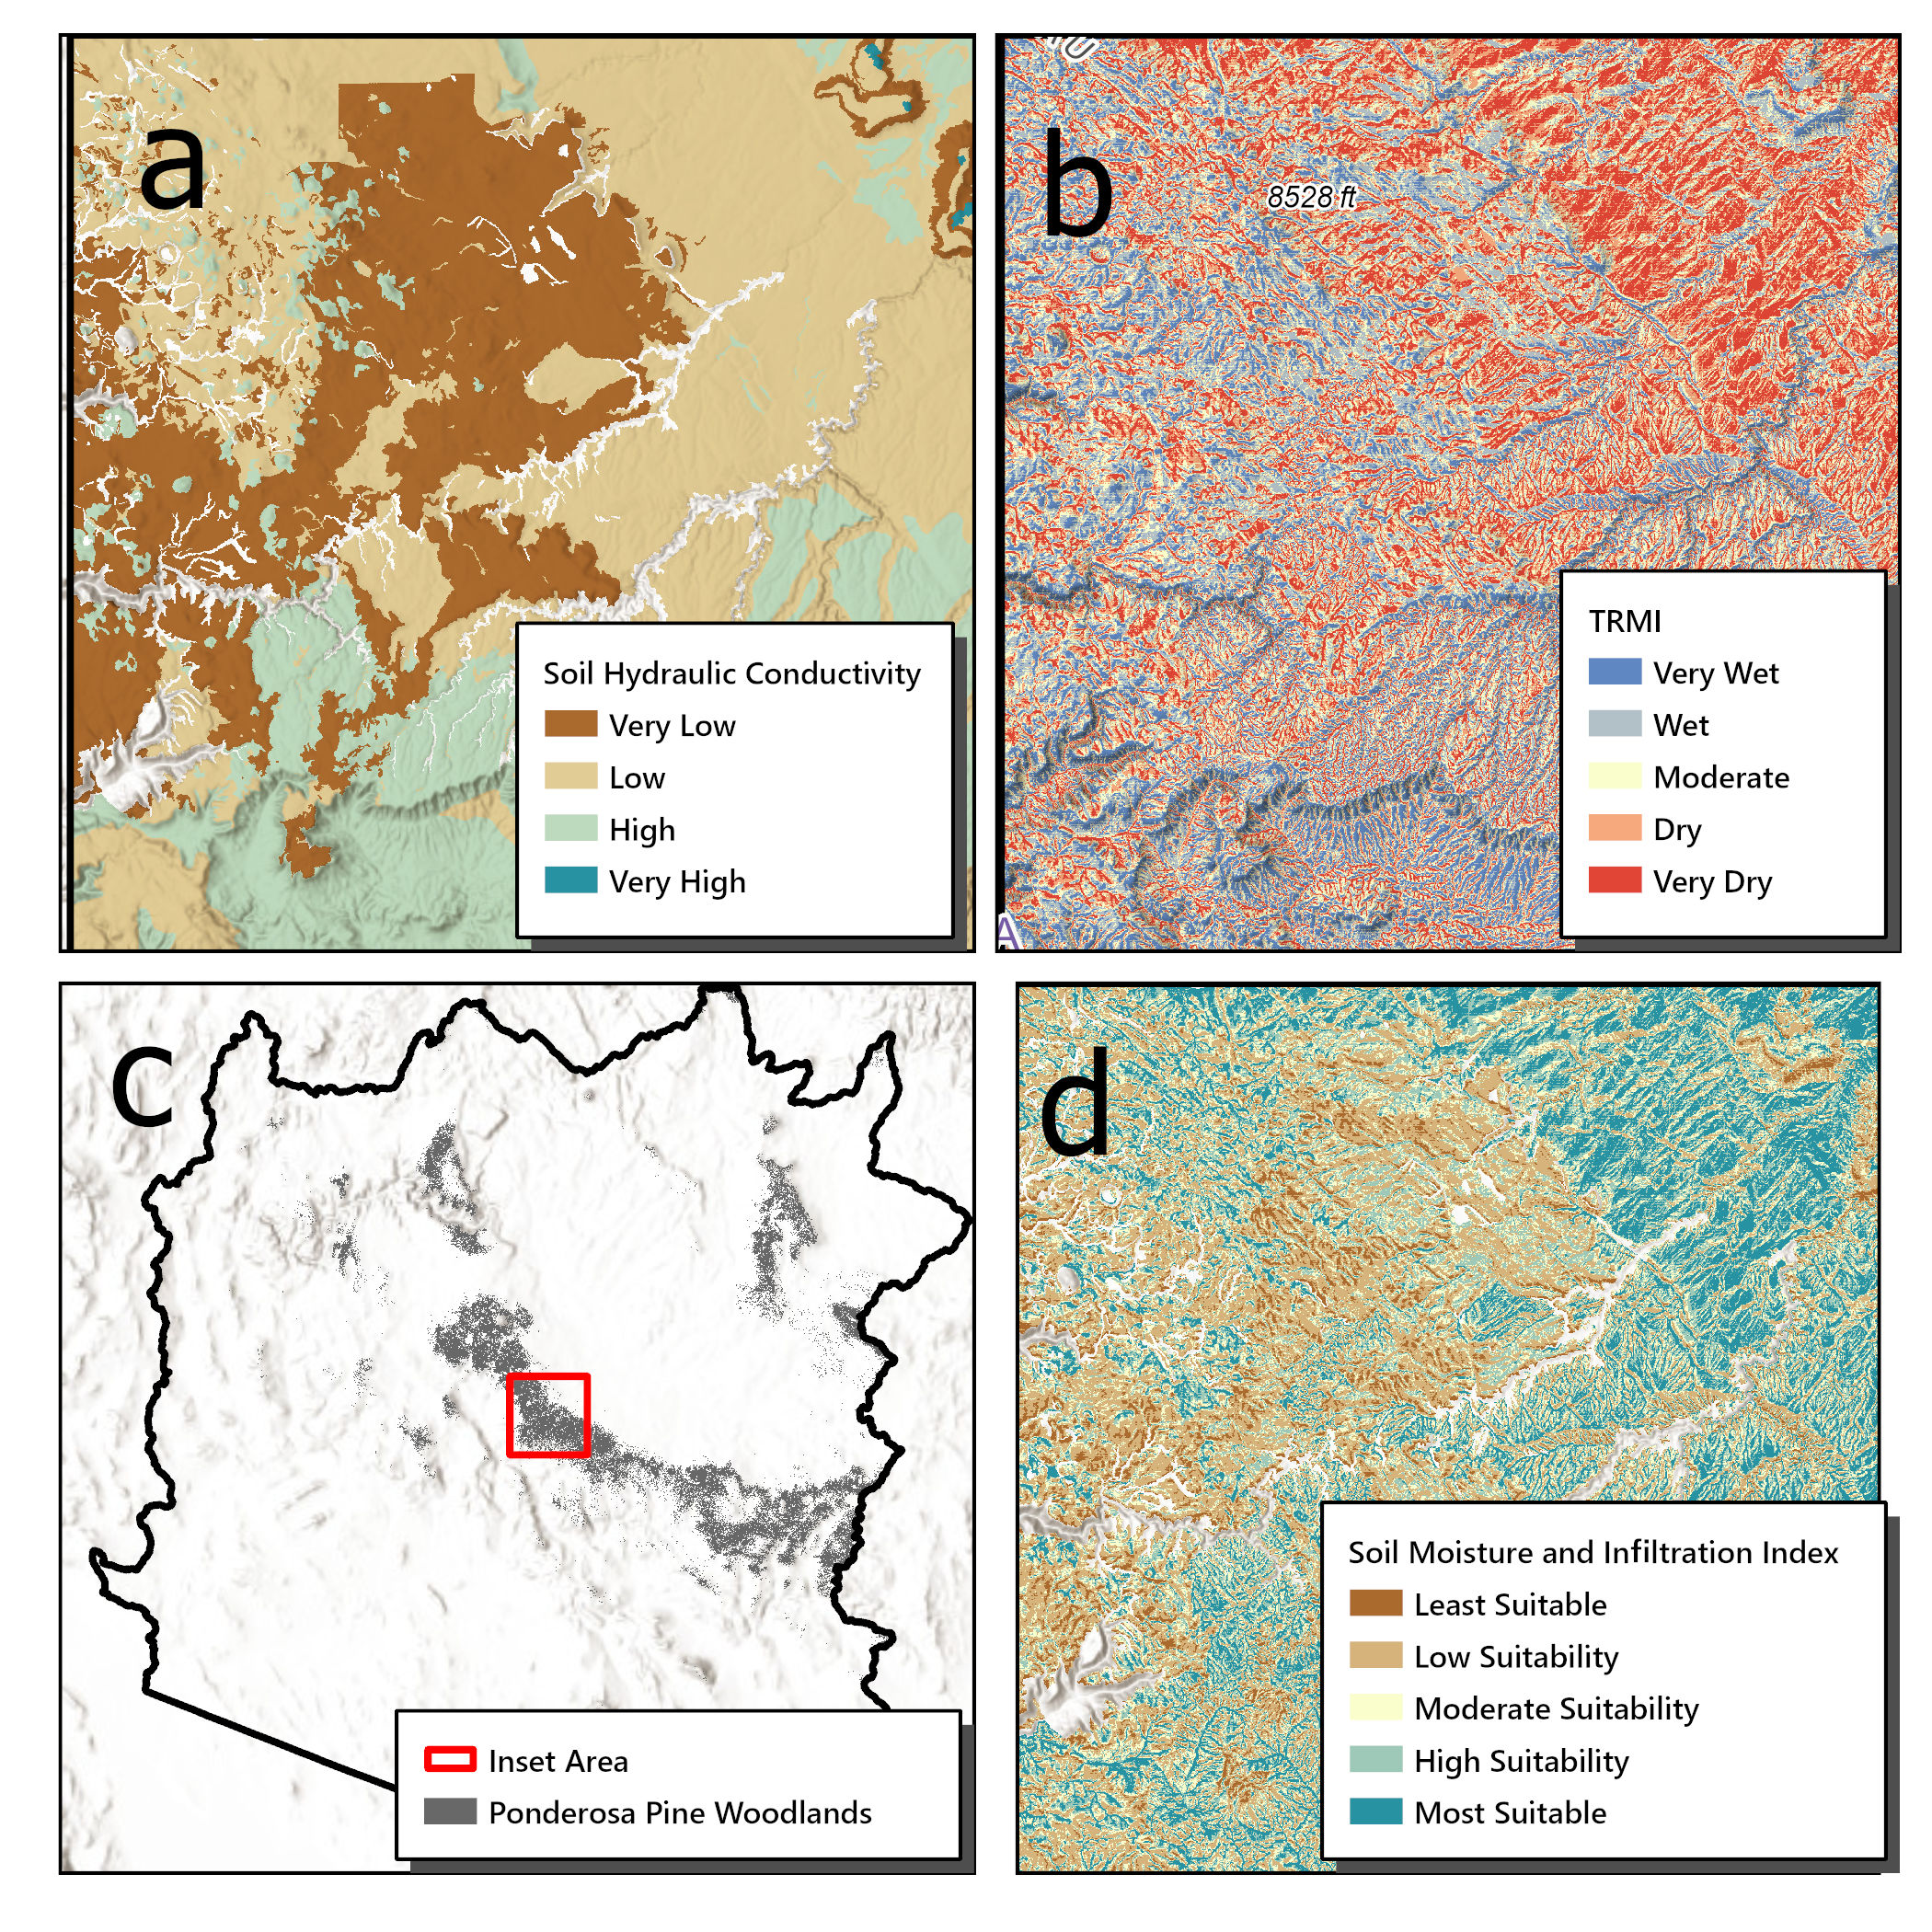
\includegraphics[keepaspectratio]{images/Soilsmap.jpg}}

}

\caption{\label{fig-soil}Panel (c) shows the zoomed in area for panels
(a),( b), and (d). Soil Moisture and Infiltration Index (d) is composed
of a weighted linear combination of Soil hydraulic Conductivity (a) and
Topographic Relative Moisture Index (b).}

\end{figure}%

\paragraph{Matrix Permeability (sPm) and Porosity
(sPo)}\label{matrix-permeability-spm-and-porosity-spo}

Permeability and Porosity values were extracted from the GLobal
Hydrogeology MaPS 2.0 (GLHYMPS v2) dataset \citep{huscroft2018}. Our
study area contained 11,057 polygons with values for saturated
log-permeability ranging from -16 to -10 and porosity values ranging
from 0.01 - 0.28 (Figure~\ref{fig-perm} ). The attribute values were
extracted, the polygons were rasterized at a 30m resolution, and then
re-scaled to values (1-10) as shown in Table~\ref{tbl-glhymps} .

\begin{longtable}[]{@{}
  >{\raggedright\arraybackslash}p{(\linewidth - 6\tabcolsep) * \real{0.2603}}
  >{\raggedright\arraybackslash}p{(\linewidth - 6\tabcolsep) * \real{0.2466}}
  >{\raggedright\arraybackslash}p{(\linewidth - 6\tabcolsep) * \real{0.2466}}
  >{\raggedright\arraybackslash}p{(\linewidth - 6\tabcolsep) * \real{0.2466}}@{}}
\caption{Classification and rescaling of GLHYMPS v2 data for suitability
mapping}\label{tbl-glhymps}\tabularnewline
\toprule\noalign{}
\begin{minipage}[b]{\linewidth}\raggedright
Log\emph{k} x 100 (Permeability)
\end{minipage} & \begin{minipage}[b]{\linewidth}\raggedright
Scaled Permeability (sPm)
\end{minipage} & \begin{minipage}[b]{\linewidth}\raggedright
Porosity x 100 (\%)
\end{minipage} & \begin{minipage}[b]{\linewidth}\raggedright
Scaled Porosity (sPo)
\end{minipage} \\
\midrule\noalign{}
\endfirsthead
\toprule\noalign{}
\begin{minipage}[b]{\linewidth}\raggedright
Log\emph{k} x 100 (Permeability)
\end{minipage} & \begin{minipage}[b]{\linewidth}\raggedright
Scaled Permeability (sPm)
\end{minipage} & \begin{minipage}[b]{\linewidth}\raggedright
Porosity x 100 (\%)
\end{minipage} & \begin{minipage}[b]{\linewidth}\raggedright
Scaled Porosity (sPo)
\end{minipage} \\
\midrule\noalign{}
\endhead
\bottomrule\noalign{}
\endlastfoot
-1650 to -1595 & 1 & 0 - 2 & 1 \\
-1595 to -1540 & 2 & 2 - 5 & 2 \\
-1540 to -1485 & 3 & 5 - 8 & 3 \\
-1485 to -1430 & 4 & 8 - 10 & 4 \\
-1430 to -1375 & 5 & 10 - 13 & 5 \\
-1375 to -1320 & 6 & 13 - 17 & 6 \\
-1320 to -1265 & 7 & 17 - 21 & 7 \\
-1265 to -1210 & 8 & 21 - 24 & 8 \\
-1210 to -1155 & 9 & 24 - 26 & 9 \\
-1155 to -1052 & 10 & 26 - 28 & 10 \\
\end{longtable}

\begin{figure}

\centering{

\pandocbounded{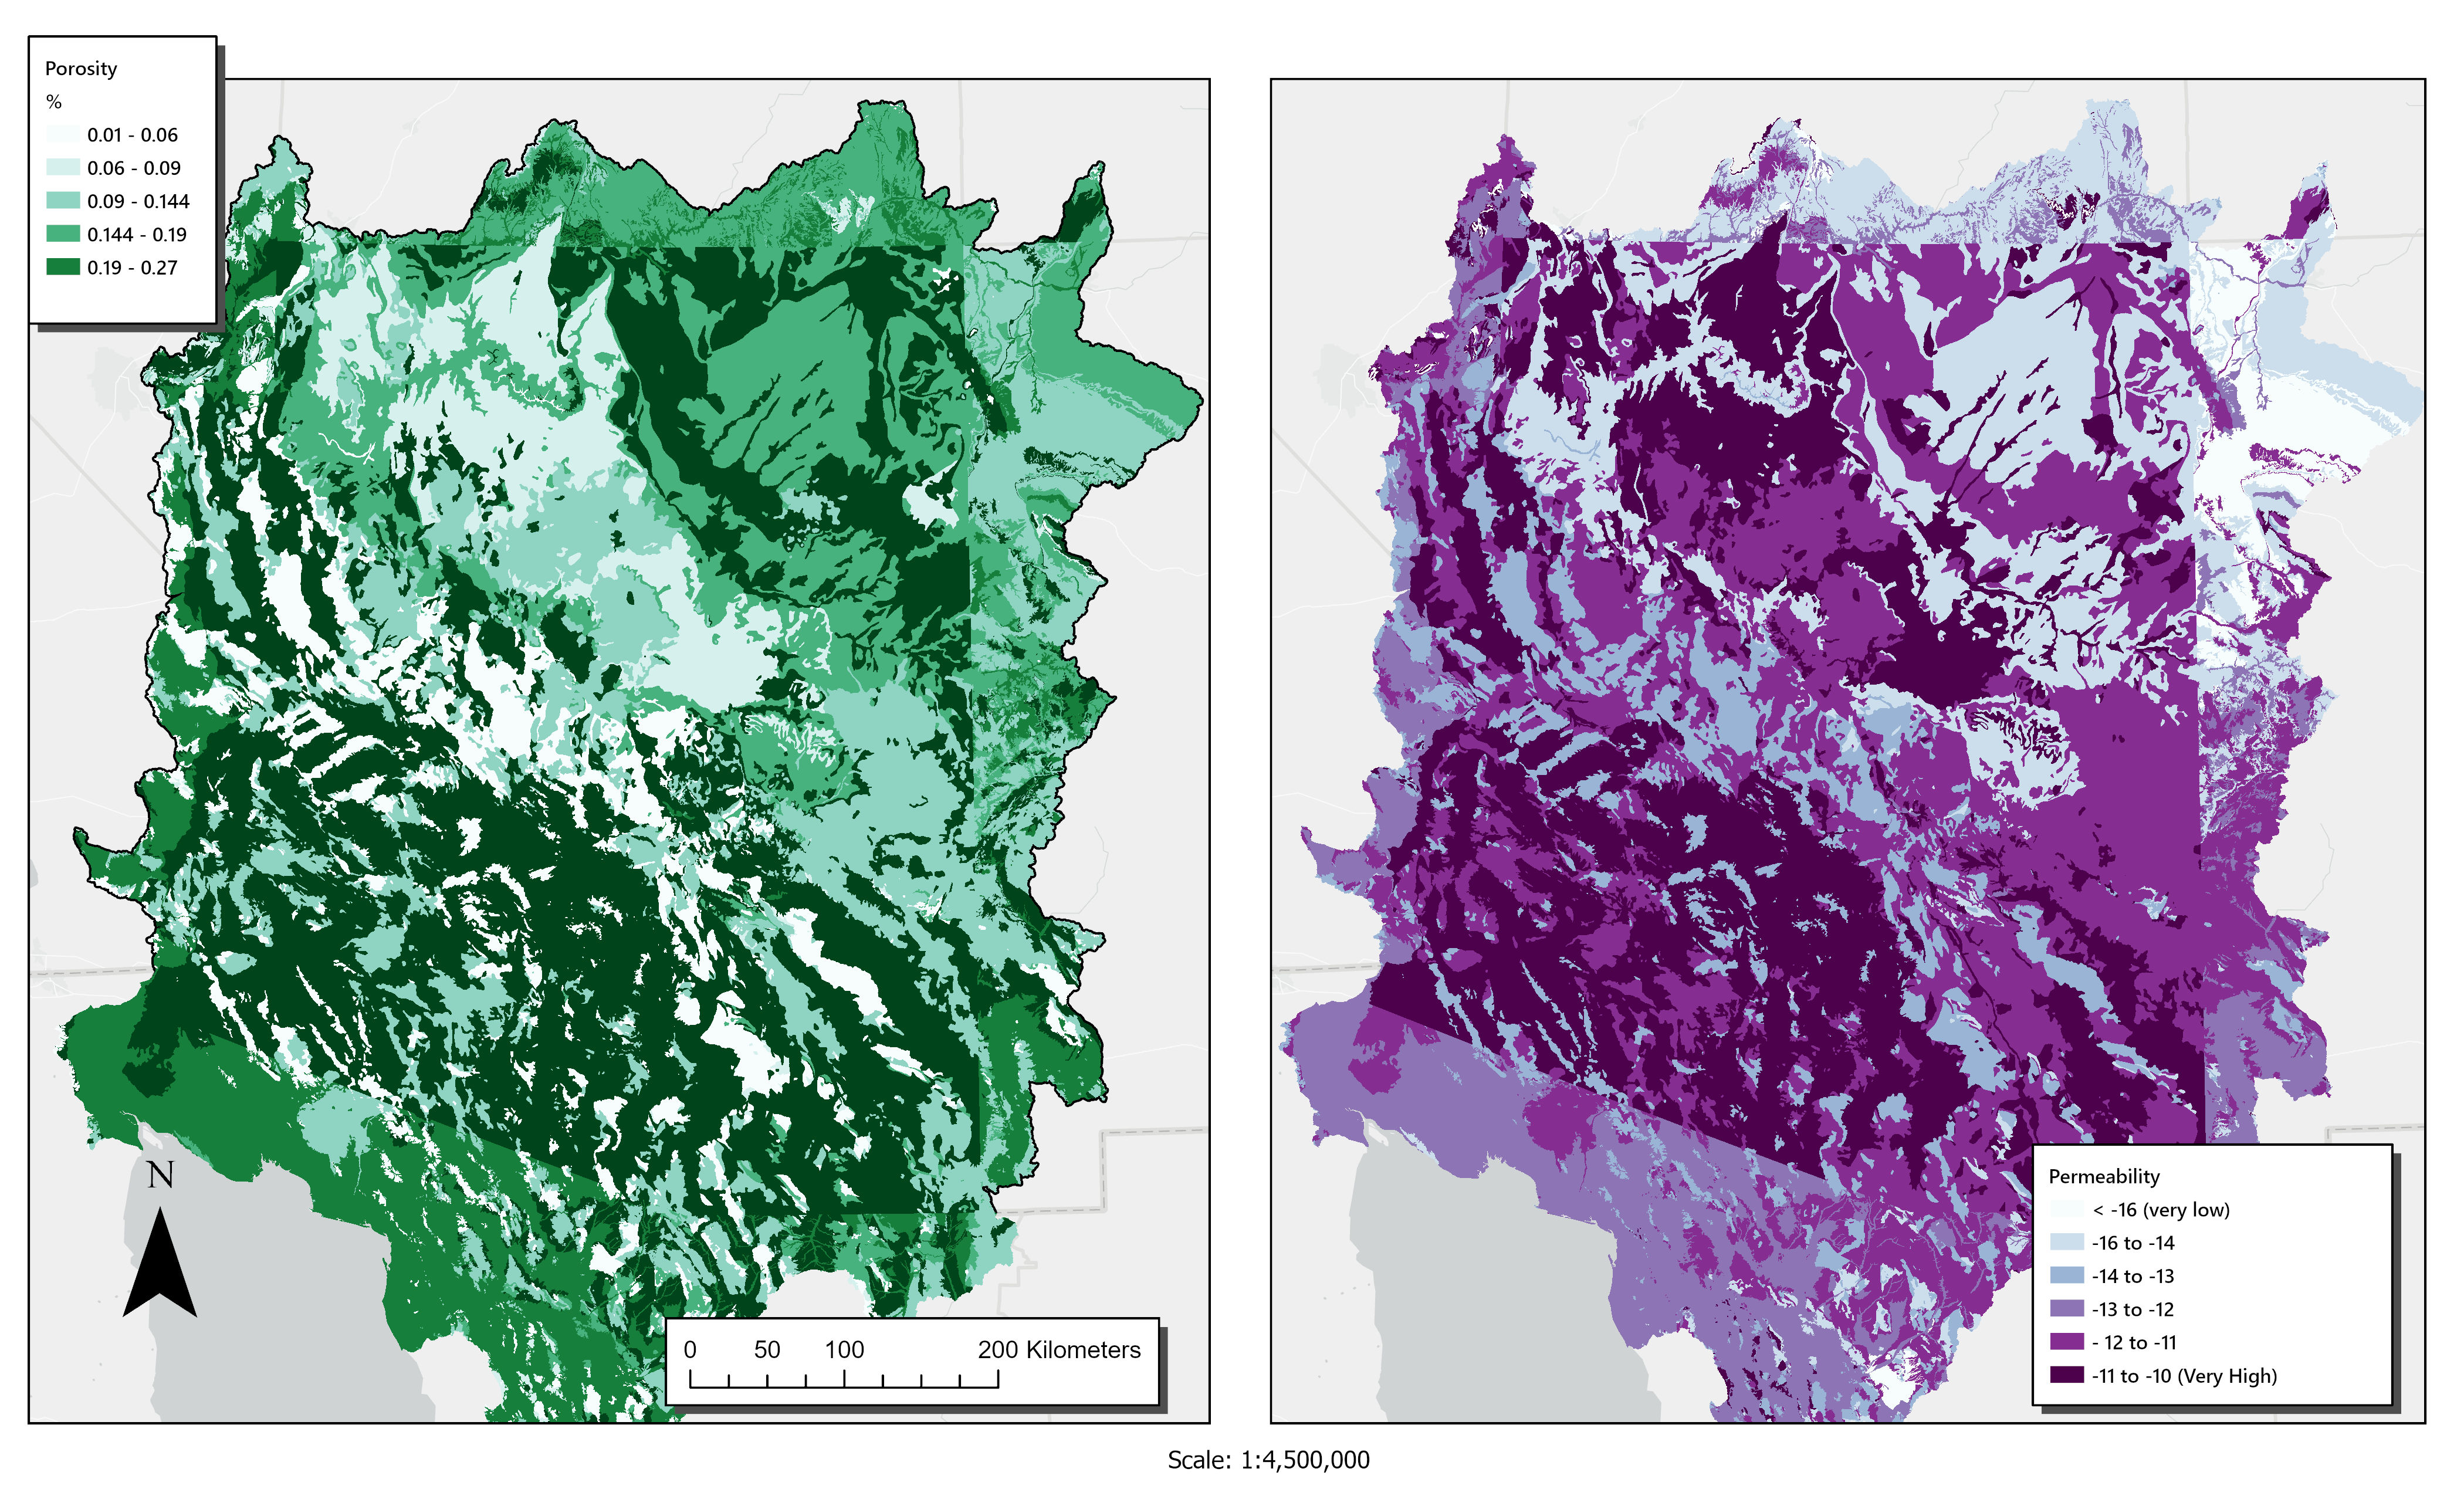
\includegraphics[keepaspectratio]{images/Geology_2_perm_porosity.jpg}}

}

\caption{\label{fig-perm}Matrix permeability and porosity values from
GLHYMPS v2 rasterized and clipped to the AZH8 Study Area}

\end{figure}%

\paragraph{Lineament Density (LD)}\label{lineament-density-ld}

Lineaments were extracted semi-automatically using 1-arc-second DEM
tiles available from the national map. Topographic Position Index (TPI)
provides estimates of relative neighborhood convexity and concavity and
was calculated using a circular neighborhood with a radius of 5m. The
TPI layer was then displayed as a multi-directional hillshade and
exported from ArcGIS to Catalyst, where the LINE module was used to
detect edges and link lines. The Default parameters were utilized, and
the resulting lineaments were brought into ArcGIS and cleaned to remove
any edge effects. A second lineament analysis was conducted using the
standard deviation of elevation with a circular neighborhood and a
radius of 5m. This raster was also displayed as a multi-directional
hillshade and exported, and lineaments were again extracted using the
LINE module. These two rasters provided complementary sets of combined
lineaments. Due to the resolution and parameters chosen, man-made
lineaments (roads, railways, and power lines) were not primarily
delineated by the algorithm in either analysis; however, buffers around
roads were randomly sampled and spot-checked to ensure man-made
lineaments were not included. The extracted lineaments are shown in
Figure~\ref{fig-linpk} . The Line Density tool in ArcGIS Pro was used to
calculate the density of lineaments using a circular neighborhood with a
radius of 1km, providing lineament density values between 0.001 and 5.55
km/km\^{}2; these values were scaled to values 1 - 10 to provide the
thematic layer Lineament Density (LD)

\paragraph{Potential Karst or Pseudo-Karst
(spK)}\label{potential-karst-or-pseudo-karst-spk}

Shapefiles of potential karst or pseudo-karst lithology were sourced
from the Karst in the United States digital map compilation and database
\citep{weary2014}. The database contains information sources from the
United States based on the State Geologic Map Compilation and maps where
lithologic units with potential for karst features at or near the
surface. The polygons were clipped to the AZHU8 study area and converted
to a 30m raster, and classified and assigned values based on their
potential for enhanced recharge through faults, fractures, sinkholes, or
caves. The classes were Non-karst = 2, Volcanics with potential karst or
pseudo--karst (such as lava tubes) = 5, Evaporites at or near the
surface = 7, and Carbonates at or near the surface = 10, resulting in a
scaled potential karst layer (spK) as shown in Figure~\ref{fig-linpk}

\begin{figure}

\centering{

\pandocbounded{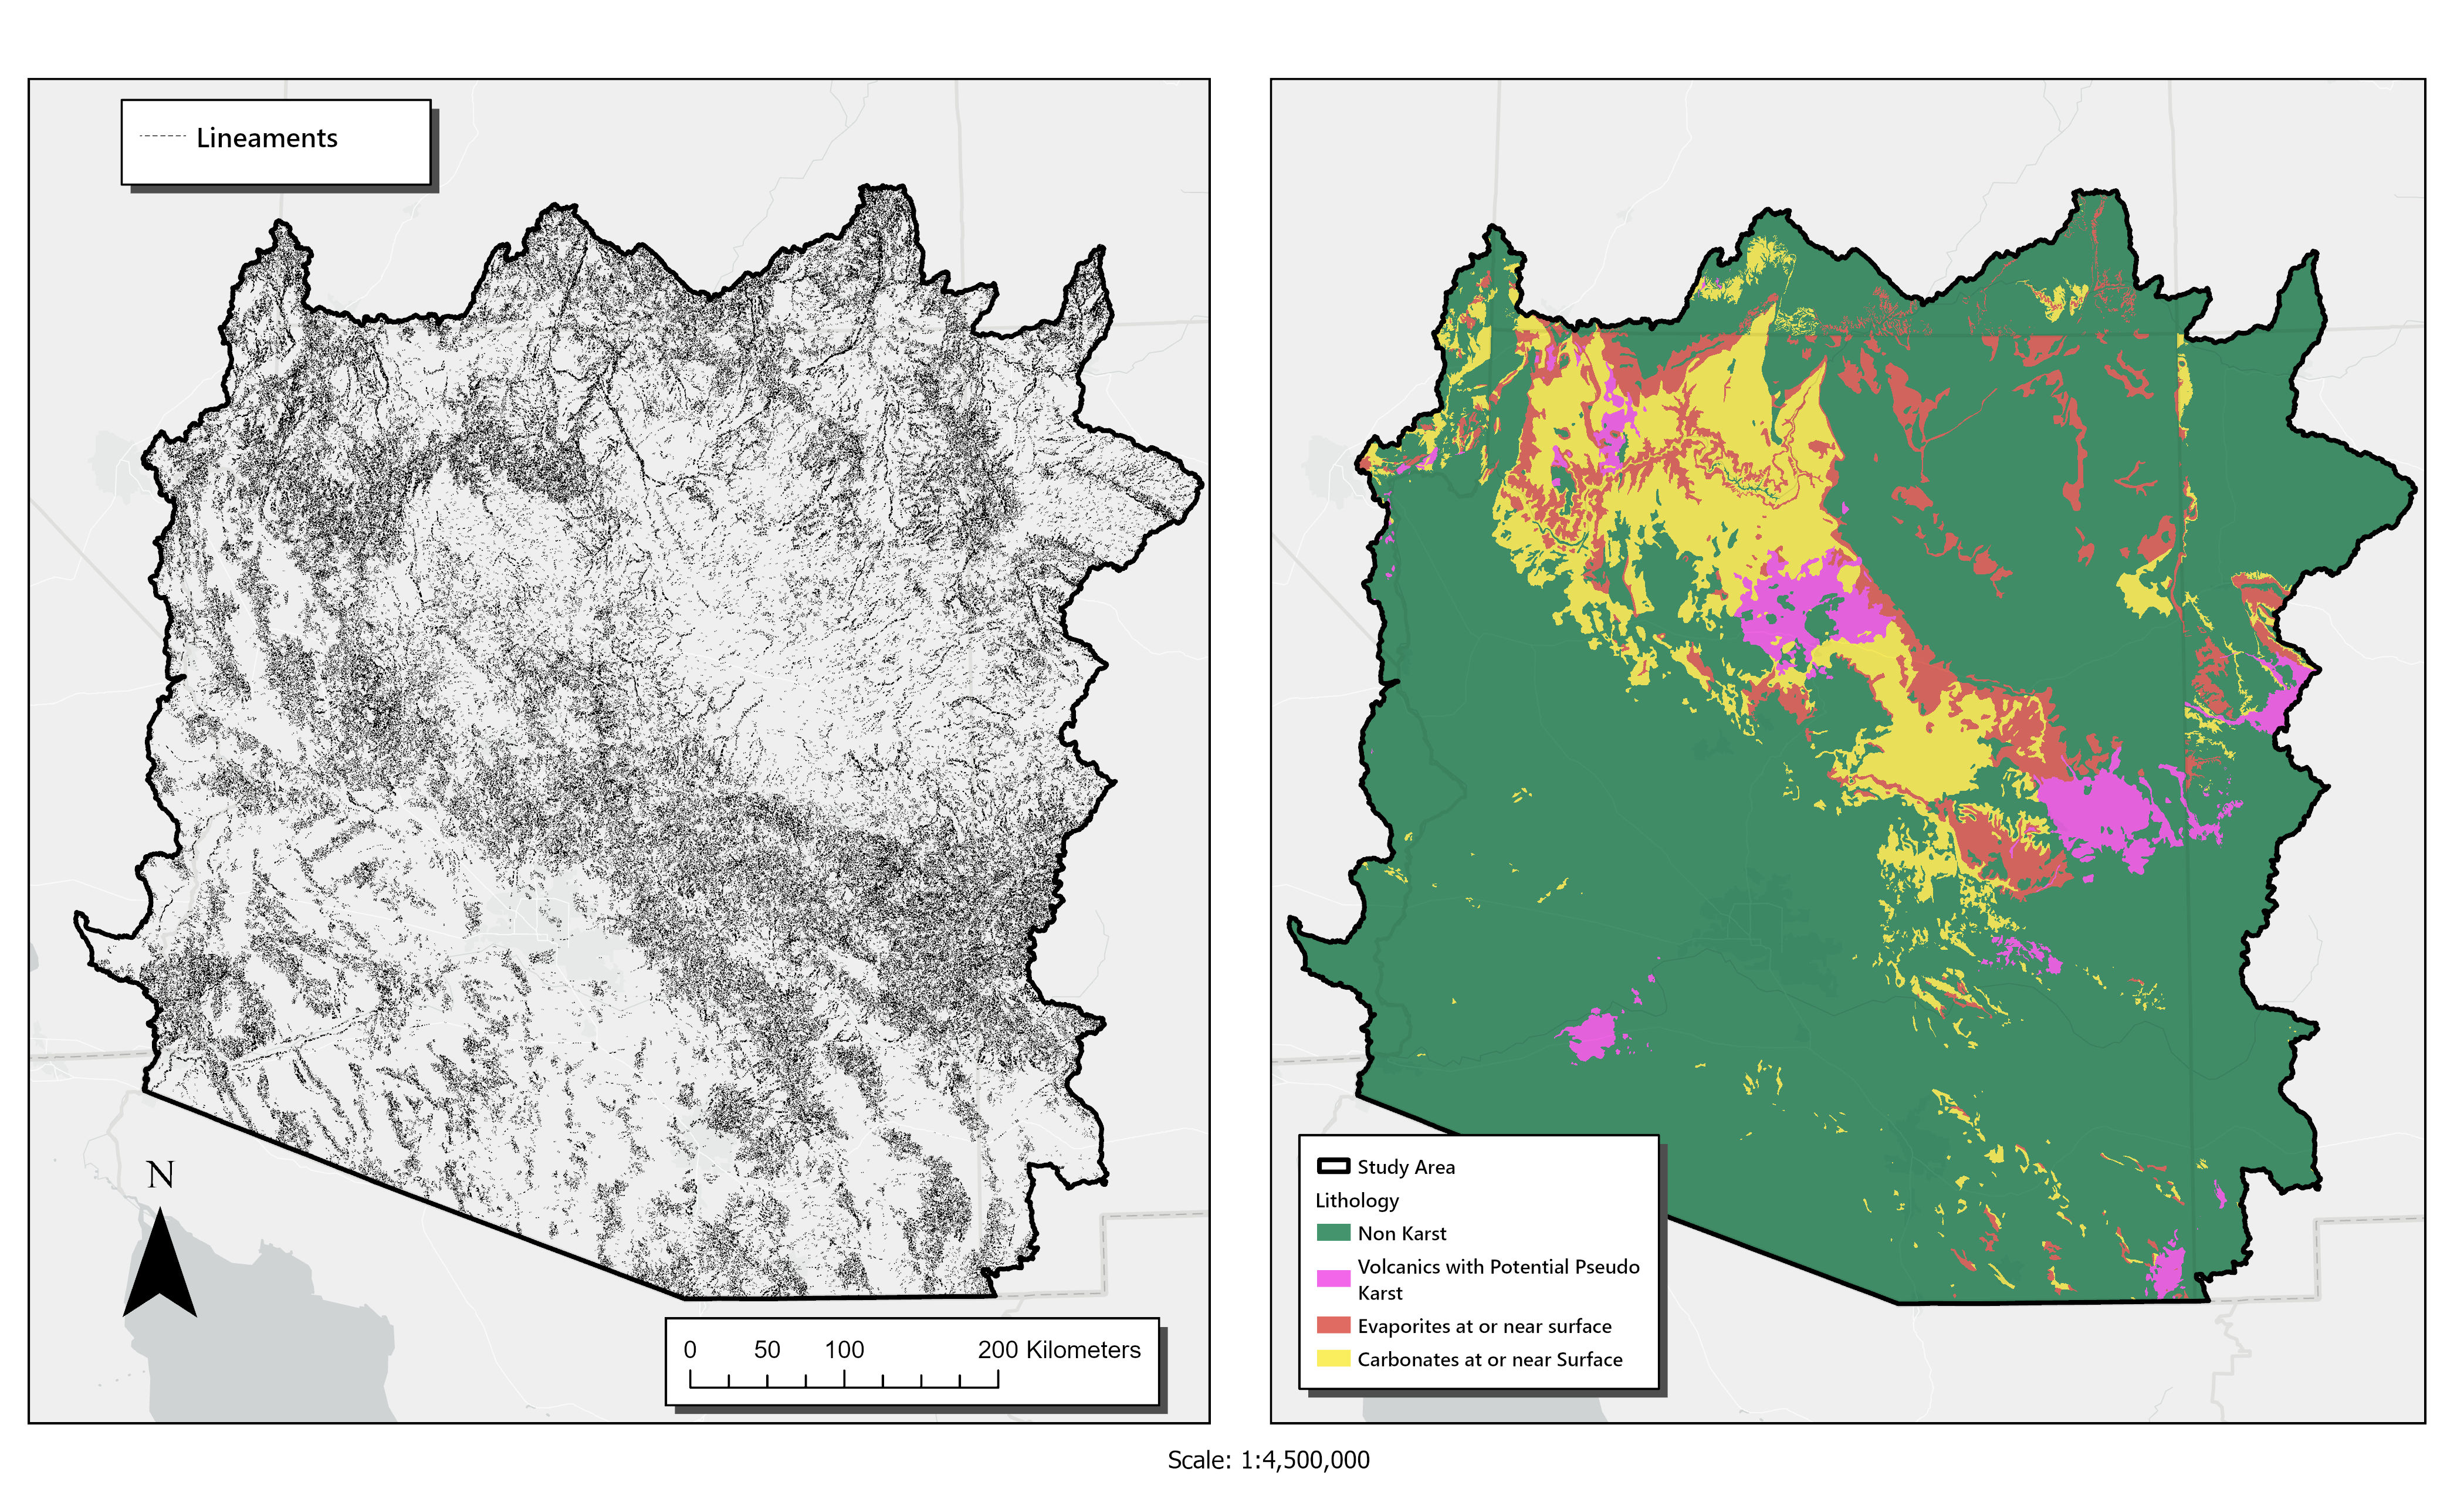
\includegraphics[keepaspectratio]{images/Geology_karst_lineaments.jpg}}

}

\caption{\label{fig-linpk}Lineaments (left) indicate fracturing, higher
secondary permeability, and porosity. Presence or Absence of karst or
Pseudo-karst (Right)}

\end{figure}%

\subsubsection{Subsurface Infiltration Index
(SbII)}\label{subsurface-infiltration-index-sbii}

This index is a weighted linear combination of sPm, sPo, LD, and sPK,
with weights 0.4, 0.25, 0.15, and 0.2 respectively, the equation is
shown below Equation~\ref{eq-Sbii}

\begin{equation}\phantomsection\label{eq-Sbii}{
SbII = ((sPm * 0.4) + (sPo * 0.25) + (LD * 0.15) + (sPK * 0.2))
}\end{equation}

\subsection{Weighting}\label{weighting}

The four final thematic layers: SF, VDI, SMII, SBII were ranked in order
of importance and assigned weights of 0.2, 0.2, 0.4, and 0.2
respectively resulting in the final suitability values for thinning to
enhance recharge shown in Equation~\ref{eq-suit} . Parameter weights and
index weights are shown in Table~\ref{tbl-w1} , Table~\ref{tbl-w2} and
\textbf{?@fig-sankey}.

\begin{equation}\phantomsection\label{eq-suit}{
Final Suitability = ((0.2 * SF) + (0.2 * VDI) + (0.4 * SMII) + (0.2 * SbII))}\end{equation}

\begin{longtable}[]{@{}
  >{\raggedright\arraybackslash}p{(\linewidth - 8\tabcolsep) * \real{0.2000}}
  >{\raggedright\arraybackslash}p{(\linewidth - 8\tabcolsep) * \real{0.2000}}
  >{\raggedright\arraybackslash}p{(\linewidth - 8\tabcolsep) * \real{0.2000}}
  >{\raggedright\arraybackslash}p{(\linewidth - 8\tabcolsep) * \real{0.2000}}
  >{\raggedright\arraybackslash}p{(\linewidth - 8\tabcolsep) * \real{0.2000}}@{}}
\caption{Table of Parameter Weights}\label{tbl-w1}\tabularnewline
\toprule\noalign{}
\begin{minipage}[b]{\linewidth}\raggedright
Total Weight
\end{minipage} & \begin{minipage}[b]{\linewidth}\raggedright
Index Weight
\end{minipage} & \begin{minipage}[b]{\linewidth}\raggedright
Sub Index Weight
\end{minipage} & \begin{minipage}[b]{\linewidth}\raggedright
Sub Sub index Weight
\end{minipage} & \begin{minipage}[b]{\linewidth}\raggedright
Parameter
\end{minipage} \\
\midrule\noalign{}
\endfirsthead
\toprule\noalign{}
\begin{minipage}[b]{\linewidth}\raggedright
Total Weight
\end{minipage} & \begin{minipage}[b]{\linewidth}\raggedright
Index Weight
\end{minipage} & \begin{minipage}[b]{\linewidth}\raggedright
Sub Index Weight
\end{minipage} & \begin{minipage}[b]{\linewidth}\raggedright
Sub Sub index Weight
\end{minipage} & \begin{minipage}[b]{\linewidth}\raggedright
Parameter
\end{minipage} \\
\midrule\noalign{}
\endhead
\bottomrule\noalign{}
\endlastfoot
20.00\% & 0.20 & - & 1.00 & Snowfall Fraction \\
13.33\% & 0.20 & - & 0.67 & Basal Area Parameter \\
6.67\% & 0.20 & & 0.33 & Canopy Cover Parameter \\
4.44\% & 0.40 & 0.67 & 0.17 & Topographic Position Index \\
8.89\% & 0.40 & 0.67 & 0.33 & Geomorphon \\
8.89\% & 0.40 & 0.67 & 0.33 & Aspect \\
4.44\% & 0.40 & 0.67 & 0.17 & Slope \\
13.33\% & 0.40 & 0.33 & 1.00 & Soil Saturated Hydraulic Conductivity \\
5.00\% & 0.20 & - & 0.25 & GLHYMPS V2 Porosity \\
8.00\% & 0.20 & - & 0.40 & GLYMPS V2 Permeability \\
3.00\% & 0.20 & - & 0.15 & Lineament Density \\
4.00\% & 0.20 & - & 0.20 & Potential Karst or Pseudo Karst \\
\end{longtable}

\begin{longtable}[]{@{}
  >{\raggedright\arraybackslash}p{(\linewidth - 6\tabcolsep) * \real{0.2740}}
  >{\raggedright\arraybackslash}p{(\linewidth - 6\tabcolsep) * \real{0.1096}}
  >{\raggedright\arraybackslash}p{(\linewidth - 6\tabcolsep) * \real{0.1096}}
  >{\raggedright\arraybackslash}p{(\linewidth - 6\tabcolsep) * \real{0.5068}}@{}}
\caption{Table of Index Weights}\label{tbl-w2}\tabularnewline
\toprule\noalign{}
\begin{minipage}[b]{\linewidth}\raggedright
Suitability Weight
\end{minipage} & \begin{minipage}[b]{\linewidth}\raggedright
Weight
\end{minipage} & \begin{minipage}[b]{\linewidth}\raggedright
Weight
\end{minipage} & \begin{minipage}[b]{\linewidth}\raggedright
Index
\end{minipage} \\
\midrule\noalign{}
\endfirsthead
\toprule\noalign{}
\begin{minipage}[b]{\linewidth}\raggedright
Suitability Weight
\end{minipage} & \begin{minipage}[b]{\linewidth}\raggedright
Weight
\end{minipage} & \begin{minipage}[b]{\linewidth}\raggedright
Weight
\end{minipage} & \begin{minipage}[b]{\linewidth}\raggedright
Index
\end{minipage} \\
\midrule\noalign{}
\endhead
\bottomrule\noalign{}
\endlastfoot
26.67\% & 0.40 & 0.67 & Topographic Relative Moisture Index \\
20.00\% & 0.20 & - & Vegetation Density Index \\
20.00\% & 0.20 & - & Subsurface Infiltration Index \\
40.00\% & 0.40 & - & Soil Moisture Infiltration Index \\
\end{longtable}

\subsection{Sensitivity Analysis}\label{sensitivity-analysis}

A sensitivity analysis was conducted on a subset of the data using a
One-at-a-time (OAT) analysis, where each parameter was systematically
removed and each index, along with the final suitability map, was
recalculated. RESULTS ARE PENDING.

\section{Results}\label{results}

The study area contained 1.8 million hectares of Ponderosa Pine forest.
Approximately 26\% (473,458 hectares) of the ponderosa pine forest was
deemed highly suitable for thinning to enhance recharge with suitability
values between 6.48 and 8.85 (out of 10); a further 33\% of the
ponderosa pine forest can be considered suitable for thinning to enhance
recharge (610,013 hectares) with suitability values between 5.42 and
6.48 (Figure~\ref{fig-finsuit} ). The remainder of the ponderosa pine
forest is moderate suitability, low suitability, or not suitable for
thinning to enhance recharge 41.28\% (761,781 hectares). Only about 3\%
of the ponderosa pine forest is classified as very high, highly
suitable, and within wilderness boundaries.

\begin{figure}

\centering{

\pandocbounded{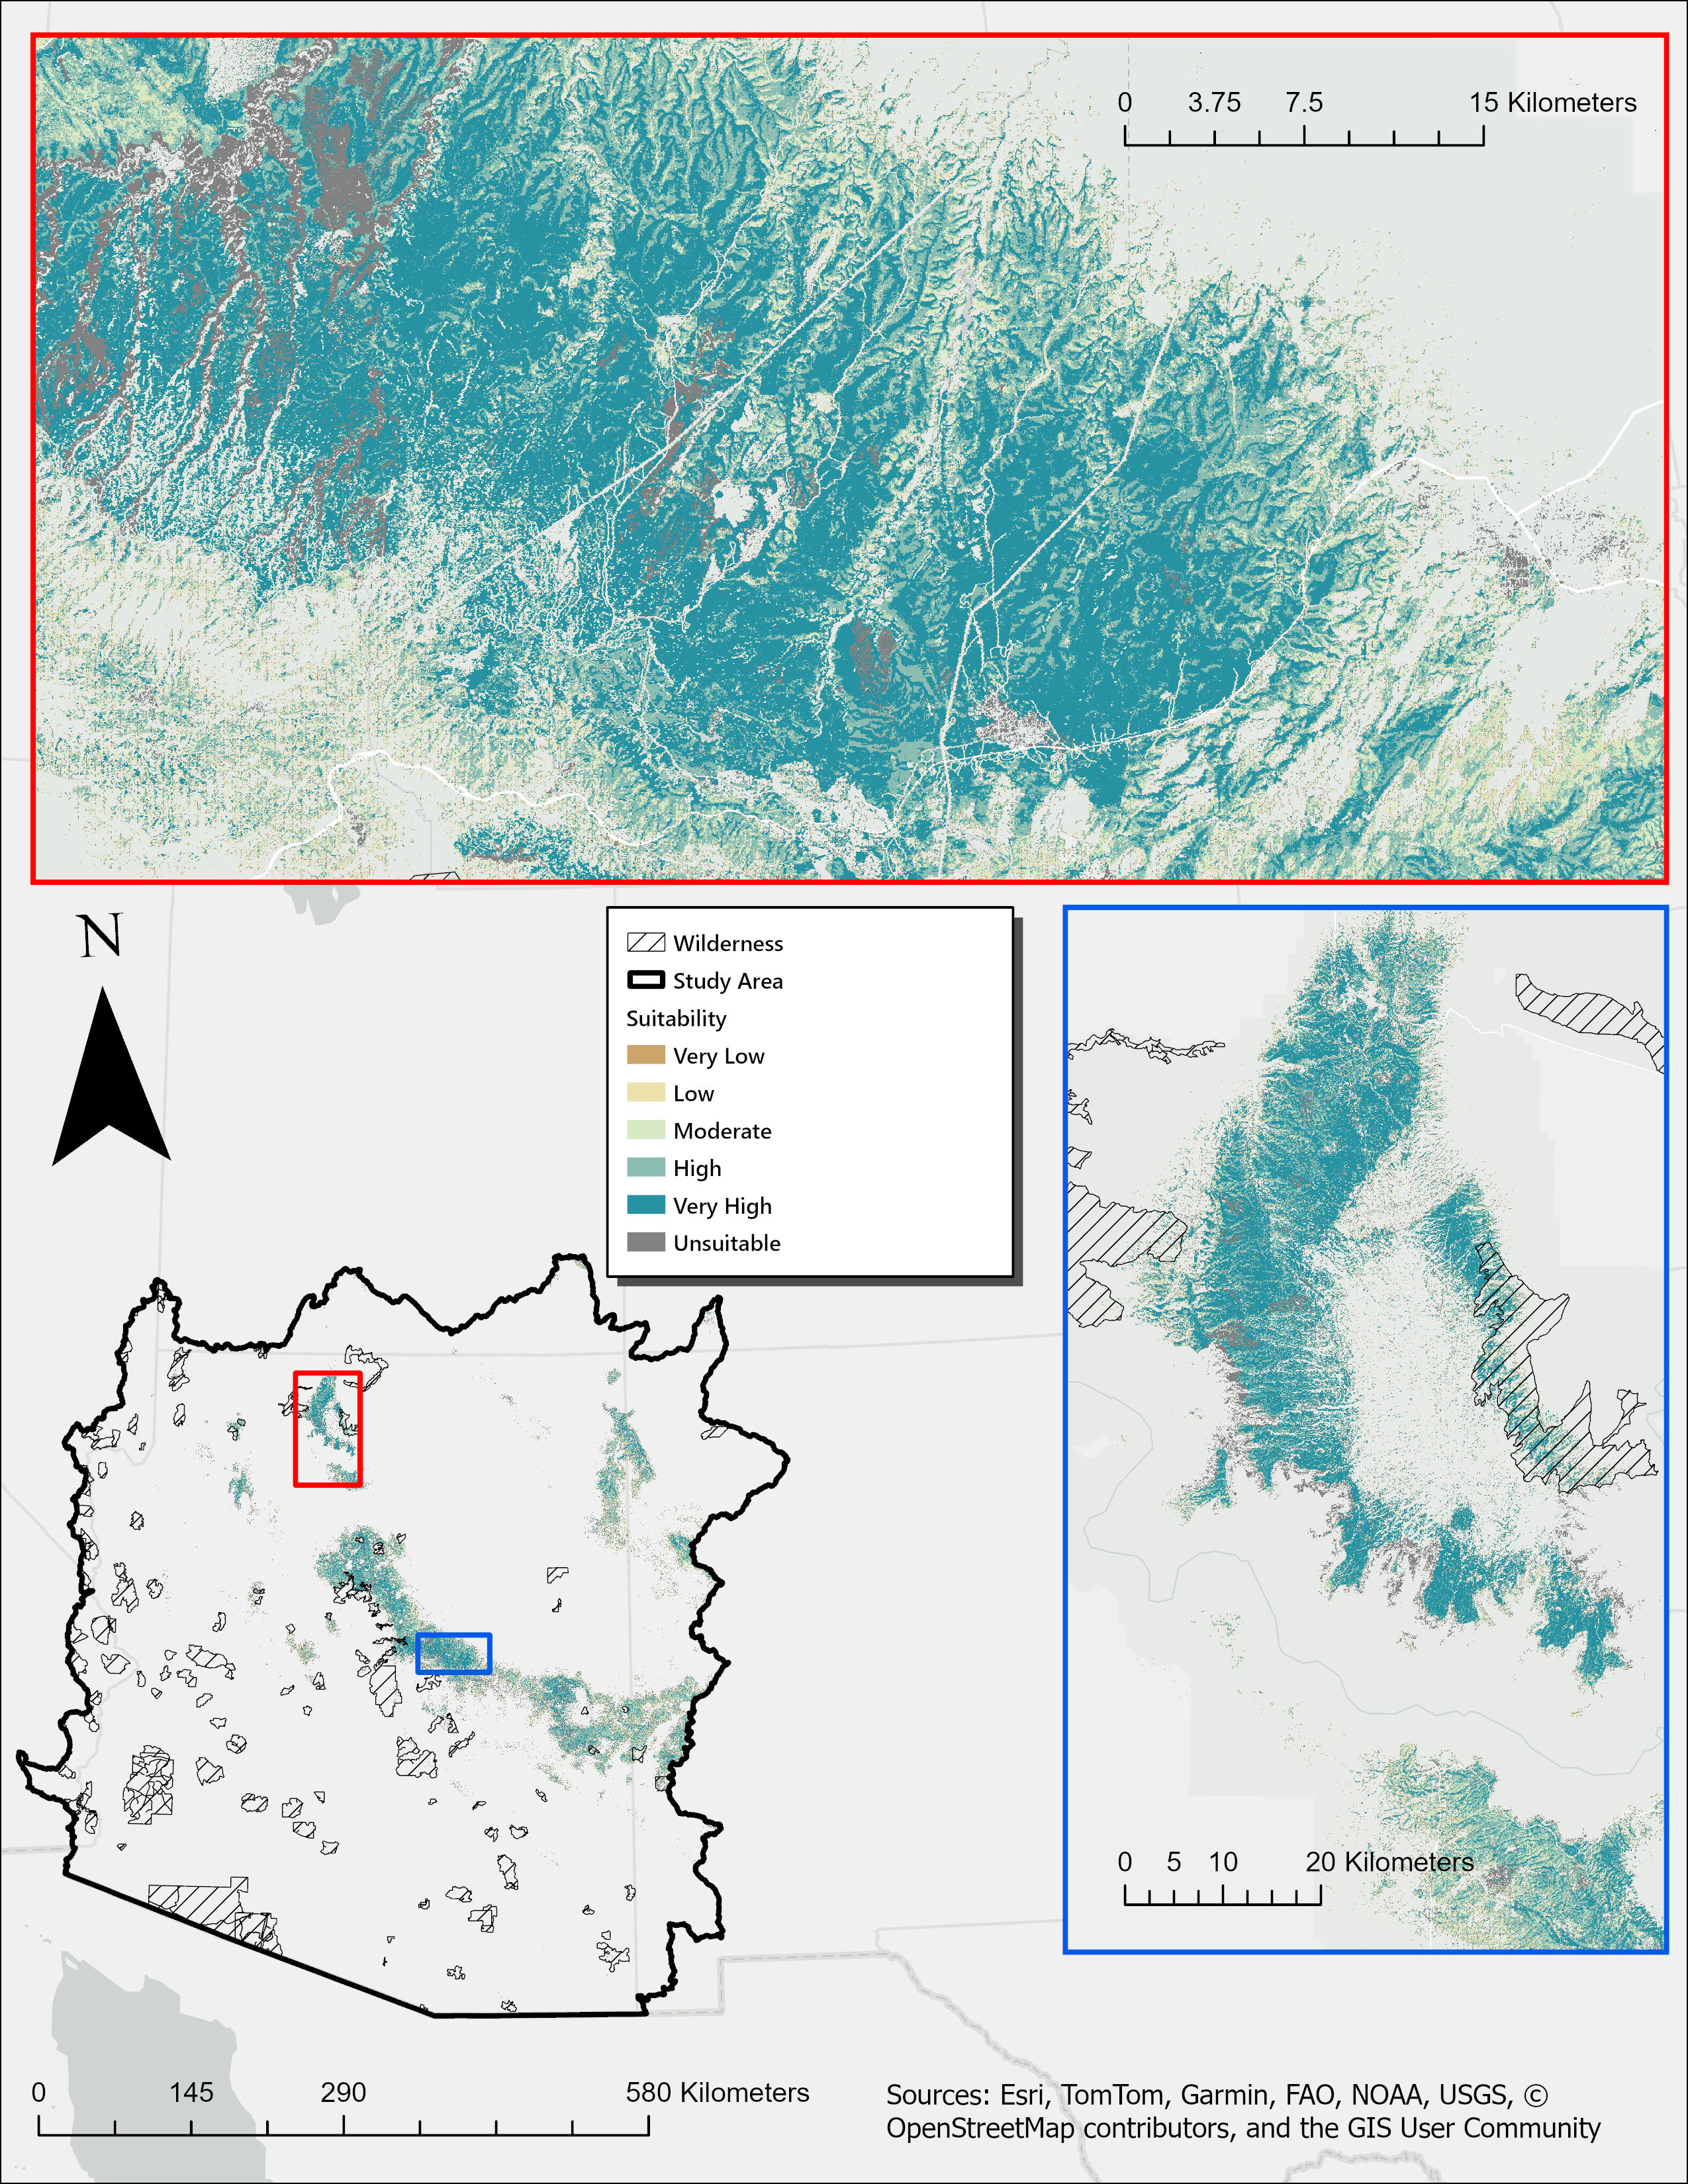
\includegraphics[keepaspectratio]{images/Statewide_suitability_Ponderosa_Pine.jpg}}

}

\caption{\label{fig-finsuit}Suitability Map for Thinning to Enhance
Groundwater Recharge}

\end{figure}%

\section{Conclusion and Discussion}\label{conclusion-and-discussion}

This research demonstrates a novel application of MCDA for mapping areas
where forest thinning could enhance groundwater recharge. The
methodology here is adaptable and could be implemented in other
semi-arid forested regions. More work is needed to validate suitability
maps using Process-Based Hydrologic Models. Groundwater is and always
has been difficult to monitor and measure. However, springs are
convenient locations to monitor the effects of land management on
groundwater recharge. Though tracer studies are needed to connect
specific springs to particular recharge areas, continuous monitoring of
springs and the base flow component of perennial spring-fed rivers can
inform land managers of the effectiveness of thinning in enhancing
recharge and help validate suitability analyses.

Forest thinning is already planned in over 1 million hectares of
Arizona's Ponderosa Pine forest. Thinning is intended primarily to
reduce the risk of catastrophic wildfire, protect forest resources,
enhance surface water provisioning and improve habitat. However, we have
also demonstrated that thinning is likely to enhance groundwater
recharge in much of the ponderosa pine forest. As water managers across
the state struggle to secure new water supplies to meet the demands of
population growth and maintain the agricultural economy, insecurity in
supplies from the Colorado River means that more and more water users
are turning to groundwater to fill the gap. Increased interest in
thinning to enhance recharge could encourage land managers to increase
the pace of restoration and find alternative funding sources for forest
restoration.

The Forest Service is mandated to manage for multiple uses; however,
groundwater recharge is not currently an explicitly managed use. In
2014, the US Forest Service introduced a proposed directive that would
mandate the consideration of groundwater resources within its
activities. However, push-back from stakeholders and state water
management agencies led to the withdrawal of this directive, with the
Forest Service vowing to start over and develop ways to include
groundwater resources within their
planning\citep{house_agriculture_committee_2014, lexology_groundwater_directive_2014, us_forest_service_2014}.
This analyses offers an avenue for considering groundwater recharge
among a host of other benefits to forests.

One of the main challenges in mapping suitability at landscape scales is
the lack of high-resolution data. Arizona lacks detailed hydrogeologic
mapping throughout much of the state. The State Geologic map within the
State Geologic Mapping Compilation contains geologic units and faults
mapped to the 1:500,000 scale. However, digitized lineaments,
particularly faults, are limited to very large faults state-wide and are
almost completely absent in the North Eastern part of the state on the
Navajo Nation and Colorado Plateau.

\section{Acknowledgments}\label{acknowledgments}

Phasellus interdum tincidunt ex, a euismod massa pulvinar at. Ut
fringilla ut nisi nec volutpat. Morbi imperdiet congue tincidunt.
Vivamus eget rutrum purus. Etiam et pretium justo. Donec et egestas sem.
Donec molestie ex sit amet viverra egestas. Nullam justo nulla,
fringilla at iaculis in, posuere non mauris. Ut eget imperdiet elit.

\section{Open research}\label{open-research}

Phasellus interdum tincidunt ex, a euismod massa pulvinar at. Ut
fringilla ut nisi nec volutpat. Morbi imperdiet congue tincidunt.
Vivamus eget rutrum purus. Etiam et pretium justo. Donec et egestas sem.
Donec molestie ex sit amet viverra egestas. Nullam justo nulla,
fringilla at iaculis in, posuere non mauris. Ut eget imperdiet elit.

\section*{References}\label{references}
\addcontentsline{toc}{section}{References}

\renewcommand{\bibsection}{}
\bibliography{bibliography.bib}





\end{document}
